\chapter{Integrationstests}

\section{Test 1 - Gleichm��iges Publizieren }
Dieser Test pr�ft ob bei Stetigem Publizieren die Frequenz korrekt Bewertet wird, und ob auf die Bewertung korrekt Reagiert wird.

\begin{enumerate}
	\item Test Launchfile starten:
	Mittels \texttt{roslaunch arni\_core test\_1\_steady.launch} wird das Launchfile gestartet.\\
	Folgende Knoten werden dabei gestartet:
	\begin{verbatim}
	    countermeasure (arni_countermeasure/arni_countermeasure)
	    ninja_turtle (arni_core/predefined_subscriber.py)
	    node_manager (arni_nodeinterface/arni_nodeinterface)
	    processing (arni_processing/arni_processing)
	    steady_tree (arni_core/predefined_publisher.py)
	\end{verbatim}
	Debei besteht folgende Verbindung der Knoten (Debugging Knoten ausgenommen f�r �bersichtlichkeit):\\

\begin{figure}[htbp]
    \begin{minipage}[t]{16cm}
        \vspace{0pt}
        \centering
        
\includegraphics[scale=0.3]{./bilder/integrationstests/test_1_nodegraph.png}
        \caption{steady\_tree publiziert mit 100Hz auf forest, ninja\_turtle aboniert forest.}
    \end{minipage}
    \hfill
\end{figure}  

    Die Frequenz von /forest wird unter 80Hz als LOW und �ber 120Hz als HIGH bewertet.
    Der Countermeasure hat das Constraint alle 10 Sekunden \textit{frequency of forest is ok} auszugeben falls die Frequenz als OK bewertet wurde.

\newpage
	\item �ffnen der GUI:
	In die Konsole wird \texttt{rosrun rqt\_gui rqt\_gui} eingegeben und ausgef�hrt.\\
	\item �ffnen der Widgets:
	Ausw�hlen des Widgets Logging->Console\\
    Debug Messages ausblenden\\

\begin{figure}[htbp]
    \begin{minipage}[t]{16cm}
        \vspace{0pt}
        \centering
        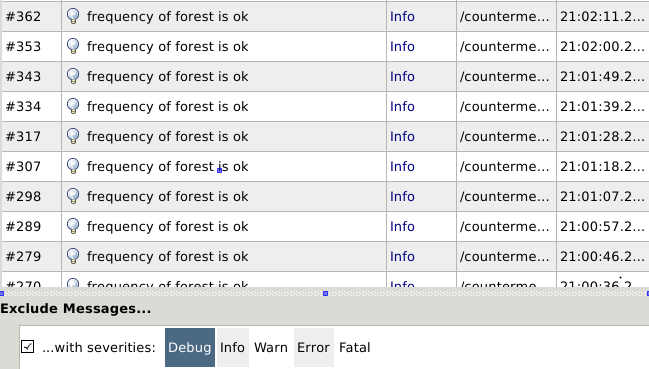
\includegraphics[scale=0.5]{./bilder/integrationstests/test_1_rqt_freq_ok.png}
        \caption{steady tree publiziert mit 100Hz auf forest. Ninja\_turtle h�rt zu.}
    \end{minipage}
    \hfill
\end{figure}  


    Es ist zu sehen das die Nachricht des Countermeasure alle 10 Sekunden publiziert wird.
\end{enumerate}